\section{Problem Description}\label{sec:prob_descr}
\subsection{Lab Setup}
\graphicspath{ {figures/} }
The helicopter, as shown on figure \ref{fig:heli1}, is constructed from two main parts. The basis and the arm. The arm has got on one side two propellers and on the opposite side a counter weight. The arm has got 2 degrees of freedom and can therefore move up and down. The two propellers are attached to the arm by a rotary bound, as shows figure \ref{fig:heli2}. 
The body of the helicopter can also rotate around its axis. Combined with the movement of the arm we observe the \textbf{travel}. The rotation of the propellers around the arm is denoted as the \textbf{pitch}. 	
\begin{figure}[h]
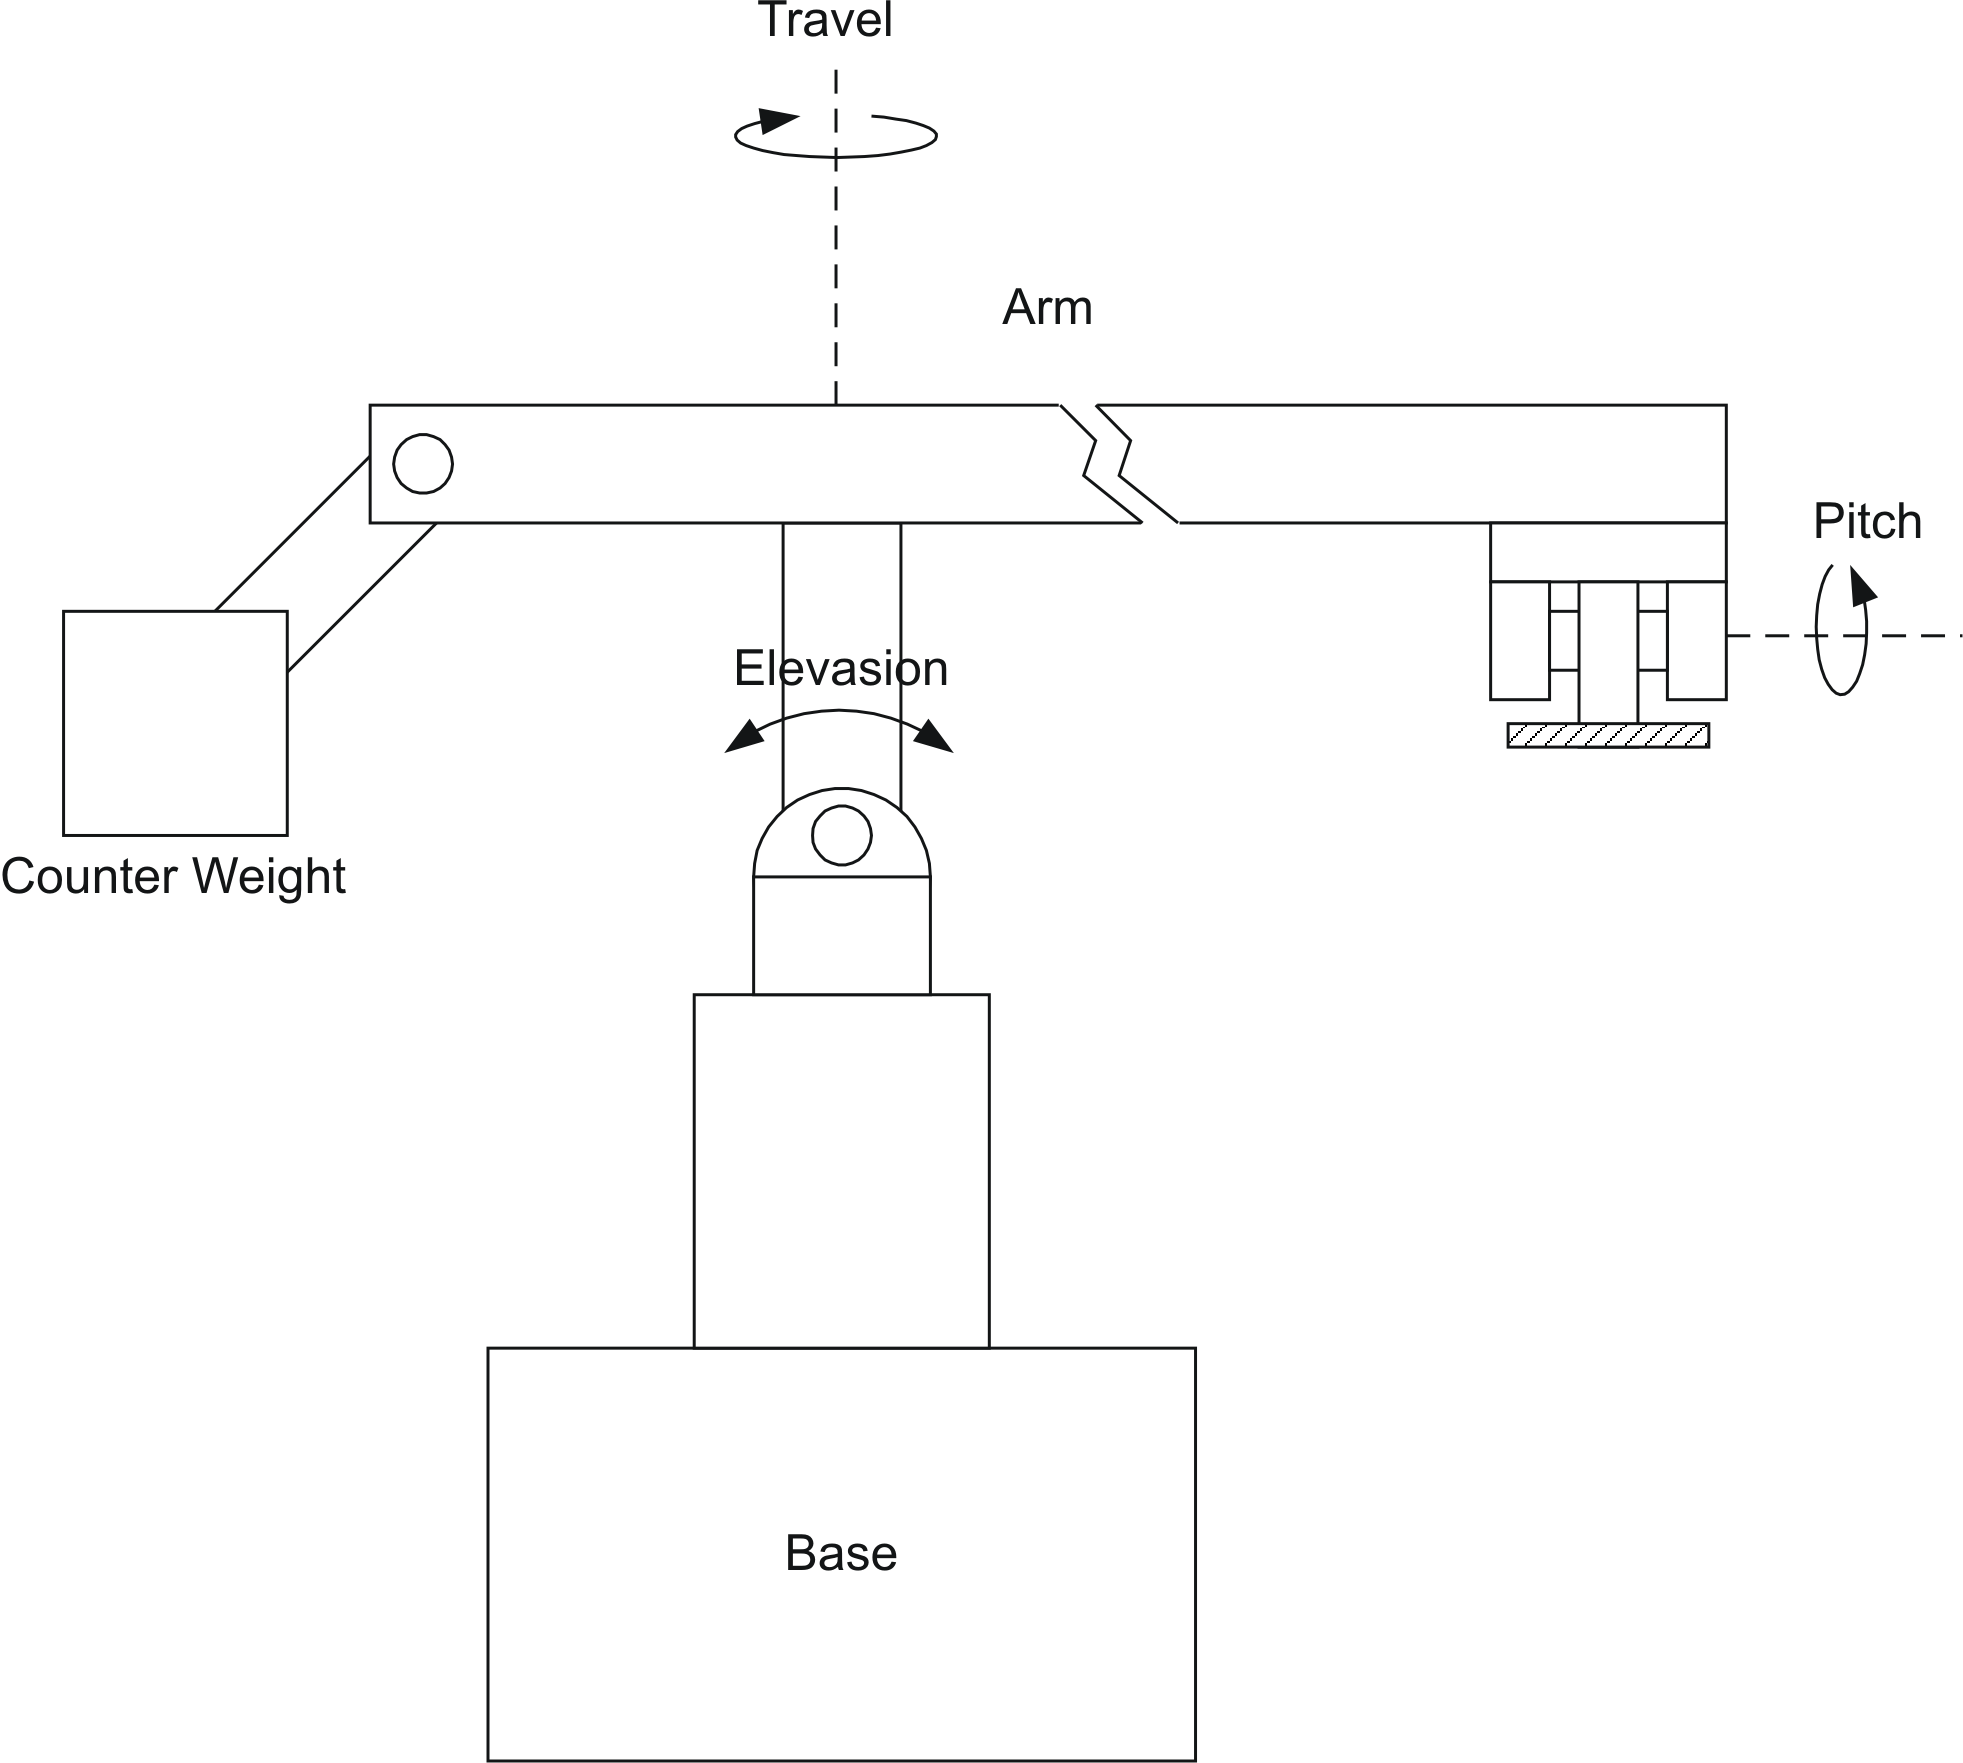
\includegraphics[width=\textwidth]{HeliScatch1.png}
\caption{the elevation of the helicopter}
\label{fig:heli1}
\end{figure} 

%\begin{figure}[h]
%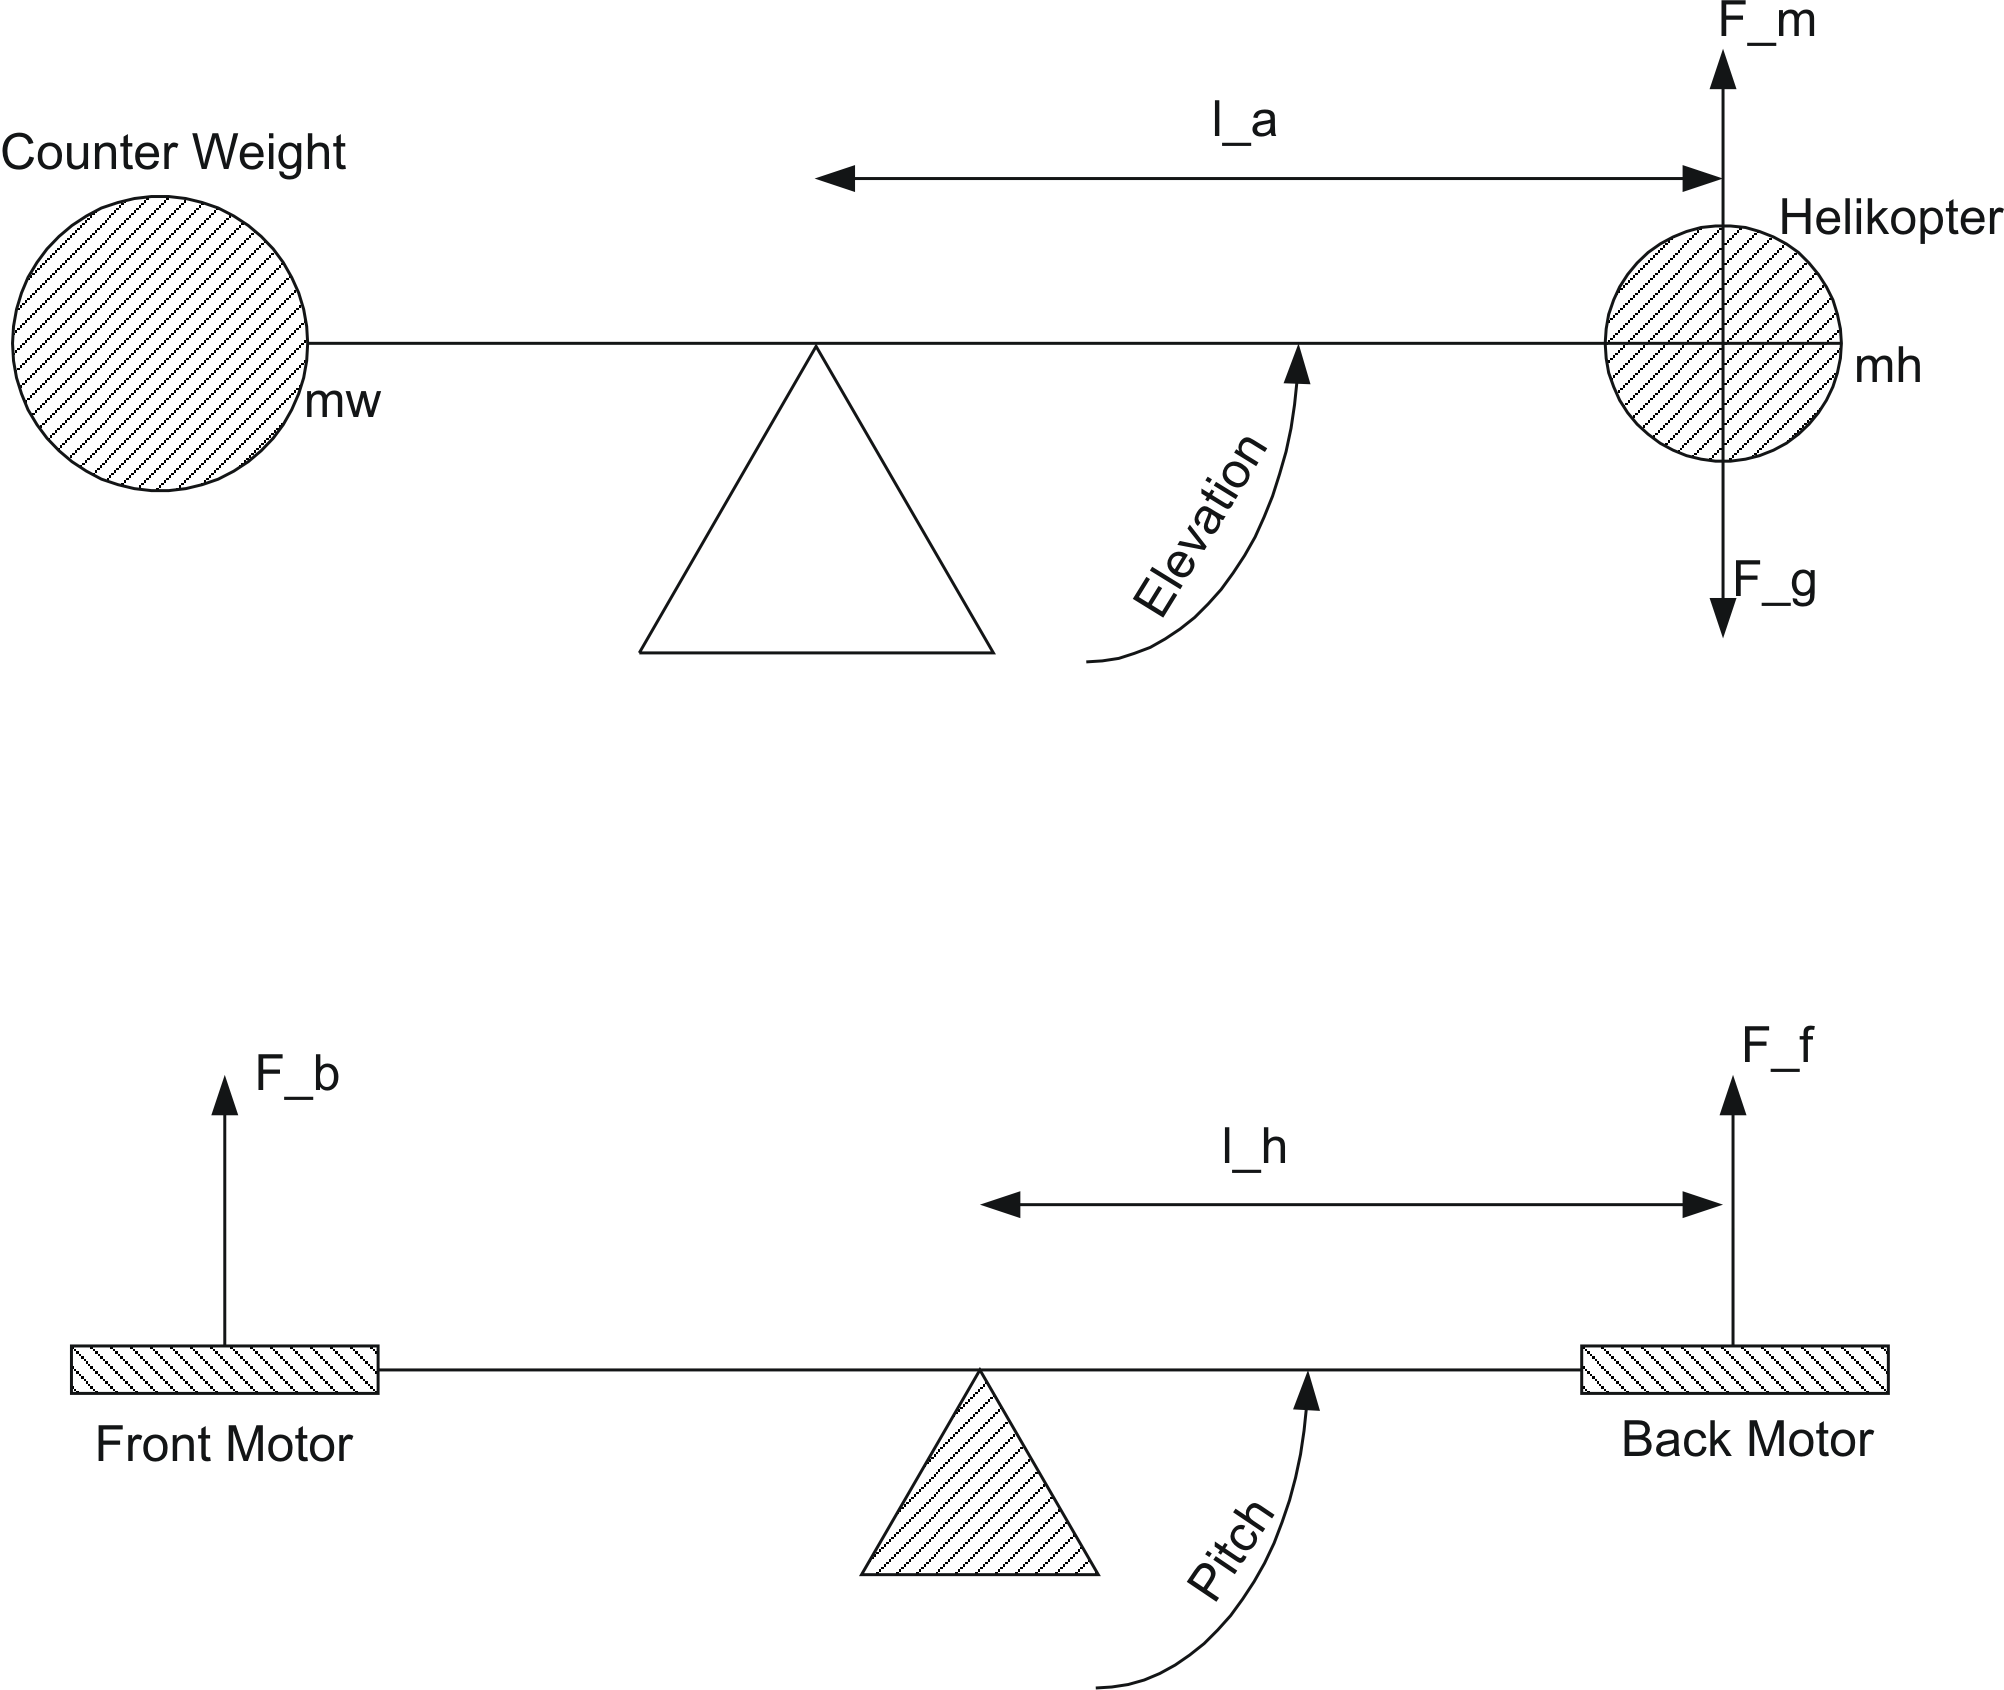
\includegraphics[\textwidth]{HeliScatch2.png}
%\caption{sketch of the helicopter}
%\label{fig:heli2}
%\end{figure}
The model is given by the quations \eqref{eq:model}. Equation \eqref{eq:model_se_al_elev} describes the elevation, equation \eqref{eq:model_se_al_pitch} accesses the pitch angle. The speed is the derivation of the of the path as described in equation \eqref{eq:model_se_al_lambda}. The travel accelaration is given by equation \eqref{eq:model_se_al_r}.  
%In this section you should describe the lab setup and discuss the model. If you want, you can copy the source code for the model equations:
%%\begin{gather}
%%	\ddot{e} + K_{3} K_{ed} \dot{e} + K_{3} K_{ep} e = K_{3} K_{ep} e_{c} \label{eq:model_elev} \\
%%	\ddot{p} + K_{1} K_{pd} \dot{p} + K_{1} K_{pp} p = K_{1} K_{pp} p_{c} \label{eq:model_pitch} \\
%%	\dot{\lambda} = r \label{eq:model_lambda} \\
%%	\dot{r} = -K_{2} p \label{eq:model_r} 
%%\end{gather}
%Since these equations belong together, it's a good idea to number them like this:    	
%\begin{subequations}
%\label{eq:model}
%\begin{gather}
%	\ddot{e} + K_{3} K_{ed} \dot{e} + K_{3} K_{ep} e = K_{3} K_{ep} e_{c} \label{eq:model_se_elev} \\
%	\ddot{p} + K_{1} K_{pd} \dot{p} + K_{1} K_{pp} p = K_{1} K_{pp} p_{c} \label{eq:model_se_pitch} \\
%	\dot{\lambda} = r \label{eq:model_se_lambda} \\
%	\dot{r} = -K_{2} p \label{eq:model_se_r} 
%\end{gather}
%\end{subequations}
%You can then both reference individual equations (``the elevation equation \eqref{eq:model_se_elev}'') or reference the entire model (``the linear model \eqref{eq:model}''). Regardless of your choice of software, never hard-code a reference, always use dynamic references. 

%You could also align the equations like this:
\begin{subequations}
\label{eq:model_al}
\begin{align}
	\ddot{e} + K_{3} K_{ed} \dot{e} + K_{3} K_{ep} e &= K_{3} K_{ep} e_{c} \label{eq:model_se_al_elev} \\
	\ddot{p} + K_{1} K_{pd} \dot{p} + K_{1} K_{pp} p &= K_{1} K_{pp} p_{c} \label{eq:model_se_al_pitch} \\
	\dot{\lambda} &= r \label{eq:model_se_al_lambda} \\
	\dot{r} &= -K_{2} p \label{eq:model_se_al_r} 
\end{align}
\end{subequations}
%You can consult \citet{Downes2002} for more about writing math.
These equations were derived from: 
\begin{equation}
	J_{2} \ddot{e} = l_{a} K_{f} V_{s} - T_{g}
	\end{equation}
s.t.
\begin{equation*}
\ddot{e}=K_{3} V_{s}-\frac{T_{g}}{J_{e}},\: K_{3}=\frac{l_{a}K_{f}}{J_{e}}.
\end{equation*}
The model is subsequently discretized into
\begin{equation*}
\Delta x_{i+1}=A\Delta x_{i} + B\Delta u_{i}
\end{equation*} 	
where
\begin{align}
\Delta x &= x -x^* \\
\Delta u &= u -u^*.
\end{align}
We want to minimize the cost function 
\begin{equation}
\phi = \sum_{i=1}^{N}(\lambda_{i}-\lambda_{f})^2+qp_{ci}^{2},\:q\geq 0
\end{equation}
\subsection{Introduction to Simulink /QuaRC}
Simulink is a program for Model-Based Design. It overtakes the code from Matlab, compiles it into the C language and sends it to the right controllers. QuaRC\footnote{\url{http://www.quarcservice.com/ReleaseNotes/files/quarc_user_guide.html}} is a Real-Time control system, that is integrated into Simulink. To control the program, Matlab and Simulink is used. We use QuaRC for the build option as can be shown on figure \ref{fig:simDiag}. 
The work flow is that we first build the program. In Simulink is than the Matlab code compiled to the C language with Visual C++. Then the code is downloaded to QuaRC. We have also to set the following parameters, if we already didn't do so, like buffer size, sampling frequency. After this, the helicopter can be started. We assure that the power button at the helicopter is on and on the computer we can push Start. After the flight, we can compare the expected flight from the real flight in a Matlab figure. The realtime measurments will always be shown up as a piece wise constant function. 
%\begin{figure}[h]
%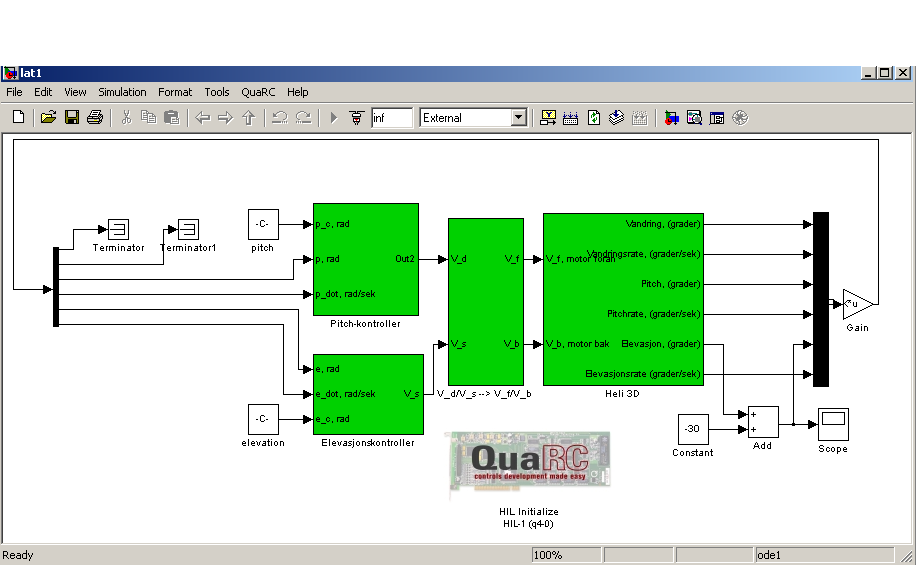
\includegraphics[\textwidth]{simulinkDiag.png}
%\caption{A diagram in Simulink.}
%\label{fig:simDiag}
%\end{figure}  
%If you decide to include a figure, that's great. You can in general copy figures from the textbook, the assignement text, or other places. However: ALWAYS CITE THE SOURCE.